
\section{图片的尺寸：包围盒与裁剪}

本节解释图片如何获得其最终尺寸。图片的尺寸即包围盒。可以限制包围盒，但在包围盒之外显示图形元素。这是 Section~\ref{sec:bb} 的主题。另一个用例是同时限制包围盒并将图形元素裁剪到某个外部路径，这是 Section~\ref{sec:clipping} 的主题。


\subsection{包围盒限制}
\label{sec:bb}

如果需要正确对齐多个图片，包围盒限制是一个有用且常常必要的工具。因此，它常与 Section~\ref{sec:pgfplots:sec:align} 的对齐方法一起使用。

包围盒限制可以通过 \PGF{} 的几种方法实现：
%
\begin{enumerate}
    \item\label{en:overlay} |overlay| 选项，
    \item |pgfinterruptboundingbox| 环境，
    \item |\pgfresetboundingbox| 命令，
    \item\label{en:useasbb} |\useasboundingbox| 路径，
    \item |trim left| 和 |trim right| 功能（这是受限包围盒和图像外部化\emph{唯一}支持的方式；至少对于 \textsc{pdf} 输出）。
        \xdef\letzterwert{\the\value{enumi}}
\end{enumerate}
%
另一个附加项是 \PGFPlots{} 的一个特定用例：
%
\begin{enumerate}
        \setcounter{enumi}{\letzterwert}
    \item |hide axis| 功能将把任何坐标轴特定内容排除在包围盒之外。详情参见 |hide axis| 的参考文档。\index{Bounding Box Control!hide axis}
\end{enumerate}

请注意，图像外部化（|external| 库）与方法 \ref{en:overlay} 到 \ref{en:useasbb} 或多或少不兼容。问题是 |pdflatex| 会裁剪掉包围盒之外的所有内容。只有两种安全方法来“限制”外部 |.pdf| 图片的包围盒：第一种是上面提到的 |trim left|/|trim right| 功能，第二种是使用负的 |\hspace| 或 |\vspace| 命令（或 |\includegraphics| 的选项）。

\begin{key}{/tikz/overlay}
        \index{Bounding Box Control!Excluding Image Parts}
    \PGF{} 的一个特殊键，它禁用图像（部分）的包围盒更新。其效果是这些部分成为文档之上的“叠加层”。

    对于 \PGFPlots{}，|overlay| 可用于将图例或其他坐标轴描述放置在坐标轴之外——而不影响其尺寸（也不影响对齐）。

    例如，人们可能想只将坐标轴的某些部分包含到最终包围盒中。这将允许水平对齐（居中）：
    %
\begin{codeexample}[]
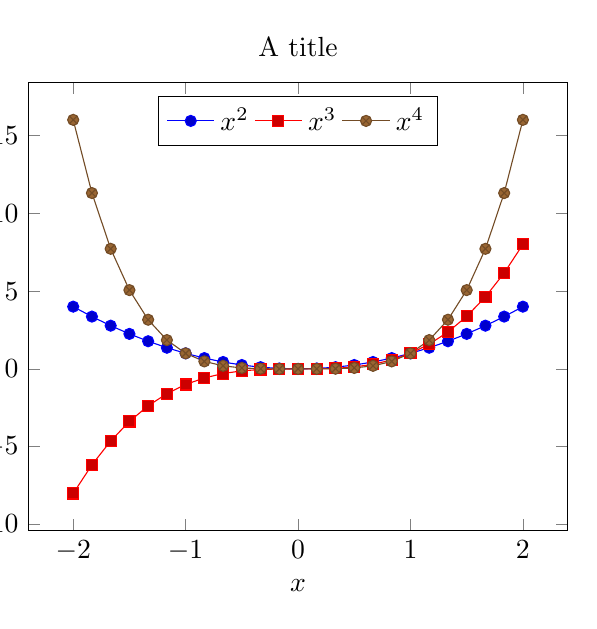
\begin{tikzpicture}
\begin{axis}[
    title=A title,
    ylabel style={overlay},
    yticklabel style={overlay},
    xlabel={$x$},
    ylabel={$y$},
    legend style={at={(0.5,0.97)},
        anchor=north,legend columns=-1},
    domain=-2:2,
]
    \addplot {x^2};
    \addplot {x^3};
    \addplot {x^4};
    \legend{$x^2$,$x^3$,$x^4$}
\end{axis}
\end{tikzpicture}
\end{codeexample}
    %
    \noindent 现在，左侧的坐标轴描述（$y$ 标签和 $y$ 刻度）伸出了包围盒。

    下面的示例将图例放置在某处，而不影响包围盒。
    %
\begin{codeexample}[]
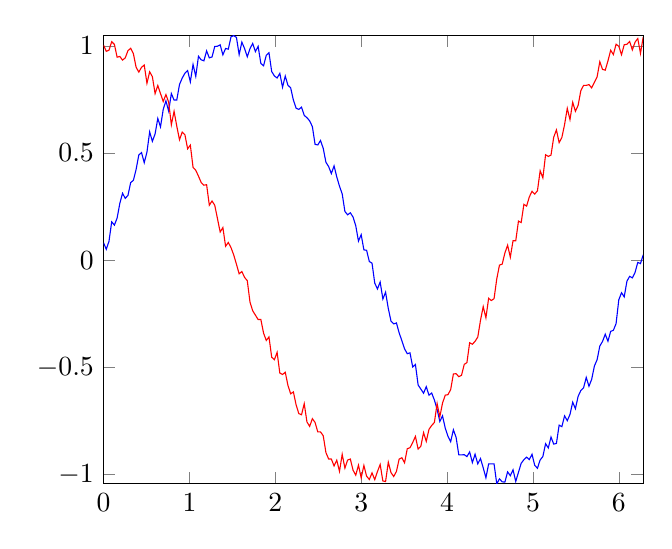
\begin{tikzpicture}
\begin{axis}[
    domain=0:6.2832,samples=200,
    legend style={
        overlay,
        at={(-0.5,0.5)},
        anchor=center},
    every axis plot post/.append style={mark=none},
    enlargelimits=false,
]
    \addplot {sin(deg(x)+3) + rand*0.05};
    \addplot {cos(deg(x)+2) + rand*0.05};
    \legend{Signal 1,Signal 2}
\end{axis}
\end{tikzpicture}
\end{codeexample}

    有关 |overlay| 选项的更多信息可在 \PGF{} 手册~\cite{tikz} 中找到。
\end{key}

\begin{command}{\pgfresetboundingbox}
    此 \pgfname{} 命令重置当前图片的包围盒。之后计算从头开始，允许计算用户定义的包围盒。
    %
\begin{codeexample}[]
\setlength{\fboxsep}{0pt}%
\fbox{%
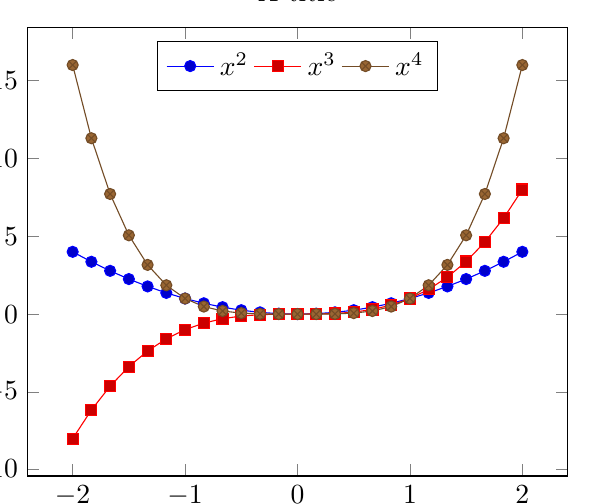
\begin{tikzpicture}
    \begin{axis}[
        title=A title,
        xlabel={$x$},
        ylabel={$y$},
        legend style={at={(0.5,0.97)},
            anchor=north,legend columns=-1},
        domain=-2:2,
    ]
        \addplot {x^2};
        \addplot {x^3};
        \addplot {x^4};
        \legend{$x^2$,$x^3$,$x^4$}
    \end{axis}

    \pgfresetboundingbox
    \path
              (current axis.south west)
    rectangle (current axis.north east);
\end{tikzpicture}%
}
\end{codeexample}
    该示例绘制一个包含坐标轴的普通图片。之后，它丢弃包围盒，并基于 |current axis| 节点及其锚点创建一个新的包围盒。
\end{command}

\begin{environment}{{pgfinterruptboundingbox}}
    \index{Bounding Box Control}
    \index{Bounding Box Control!pgfinterruptboundingbox}

{
        \pgfmanualpdflabel{\textbackslash useasboundingbox}{}
    下面展示另一种具有相同效果的方法：手动中断包围盒，之后再恢复。
    %
\begin{codeexample}[]
\setlength{\fboxsep}{0pt}%
\fbox{%
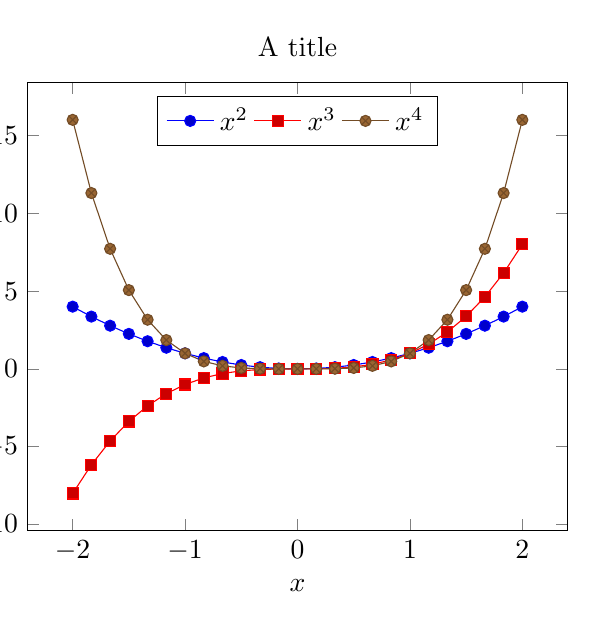
\begin{tikzpicture}
  \begin{pgfinterruptboundingbox}
    \begin{axis}[
        title=A title,
        xlabel={$x$},
        ylabel={$y$},
        legend style={at={(0.5,0.97)},
            anchor=north,legend columns=-1},
        domain=-2:2,
    ]
        \addplot {x^2};
        \addplot {x^3};
        \addplot {x^4};
        \legend{$x^2$,$x^3$,$x^4$}
    \end{axis}
  \end{pgfinterruptboundingbox}

    \useasboundingbox
                  (current axis.below south west)
        rectangle (current axis.above north east);
\end{tikzpicture}%
}
\end{codeexample}
}
    %
    |pgfinterruptboundingbox| 环境不将其内容包含到图像的包围盒中，而 |\useasboundingbox| 将图片包围盒设置为以下参数（参见~\cite{tikz}）。
\end{environment}

\begin{keylist}{%
    /tikz/trim left=\marg{$x$-coordinate or point} (default 0pt),
    /tikz/trim right=\marg{$x$-coordinate or point}%
}
    这两个键允许减小包围盒的尺寸。

    |trim left| 键期望一个单一 $x$ 坐标（如 |1cm|）或一个点（如 |(current axis.west)|）。如果提供了点，它只使用该点的 $x$ 坐标。然后，包围盒的左端设置为得到的 $x$ 坐标，其左侧的所有内容都在包围盒之外。

    |trim right| 键具有相同效果，只是用于包围盒的右端。

    更详细的文档可在 \Tikz{} 手册中找到。
\end{keylist}

\begin{stylekey}{/tikz/trim axis left}
    一个值为 |trim left=(current axis.south west)| 的样式。

    此样式需要作为参数提供给 |\begin{tikzpicture}[trim axis left]|。它期望图片中（至少）有一个 \PGFPlots{} 环境。其效果是修剪最后一个坐标轴锚点 |south west| 左侧的所有内容（即左坐标轴边界左侧的所有内容）。
\end{stylekey}

\begin{stylekey}{/tikz/trim axis right}
    一个值为 |trim right=(current axis.south east)| 的样式。

    它的工作方式与 |trim axis left| 类似：其效果是最后一个坐标轴环境的右坐标轴线右侧的所有内容都从包围盒中截断。
\end{stylekey}

\begin{stylekey}{/tikz/trim axis group left}
    一个与 |trim axis left| 效果相同但为 |groupplots| 库量身定制的样式。

    它的值为 |trim left=(group c1r1.south west)|。

    此样式需要作为参数提供给 |\begin{tikzpicture}[trim axis group left]|。它期望图片中（至少）有一个 |groupplot| 环境。其效果是修剪第一个组坐标轴锚点 |south west| 左侧的所有内容（即左坐标轴边界左侧的所有内容）。
\end{stylekey}

\begin{stylekey}{/tikz/trim axis group right}
    一个与 |trim axis right| 效果相同但为 |groupplots| 库量身定制的样式。

    它的工作方式与 |trim axis group left| 类似：其效果是组图中最右侧坐标轴（|groupplot| 环境的最后一个元素）右侧的所有内容都从包围盒中截断。
\end{stylekey}


\subsection{裁剪}
\label{sec:clipping}

与包围盒限制（在保持相同图形输出的同时减小图片最终尺寸）不同，裁剪同时影响图片尺寸和可见输出。

通常，\PGFPlots{} 使用带框坐标轴的路径作为裁剪路径。然而，裁剪有一些特殊功能和微调键，本节将解释。

\begin{pgfplotskey}{clip=\mchoice{true,false} (initially true)}
        \index{Bounding Box Control!clip}
    控制坐标轴内部的任何路径是否应被裁剪。

    即使 |hide axis=true|，这仍然有效。

    请注意，裁剪路径可以对图片的包围盒产生贡献。从 |compat=1.8| 开始，\PGFPlots{} 应用智能来分离裁剪和包围盒控制的职责，参见 |clip bounding box| 及其选项。自 |compat=1.8| 起，即使包围盒远小于裁剪路径，裁剪路径仍可生效。如果裁剪路径不可见，这通常就是人们所期望的。

    裁剪路径使用 |\pgfplotspathaxisoutline| 生成，即它是由带框坐标轴线引出的路径。对于三维图，仅使用外部坐标轴线。具有居中标轴线的图也使用外部坐标轴线。
\end{pgfplotskey}

\begin{pgfplotskey}{clip marker paths=\mchoice{true,false} (initially false)}
    初始选项 |clip marker paths=false| 使标记在裁剪区域\emph{之后}绘制。只有它们的位置会被裁剪。

    因此，标记要么完全绘制，要么根本不绘制。值 |clip marker paths=true| 是为了向后兼容：它不引入特殊的标记处理，因此如果标记靠近裁剪边界，可能会被部分绘制。\footnote{请注意，裁剪后的标记路径在 \TeX{} 编译期间可能略快。}

    如果 |clip=false|，此键无效。

    请注意，裁剪标记路径还影响图及其标记相互重叠绘制的顺序。另请参阅相关键 |clip mode|。
\end{pgfplotskey}

\begin{pgfplotskey}{%
    clip bounding box=\mchoice{default tikz,upper bound} (initially controlled by compat key)%
}
    控制由 |clip=true| 生成的路径如何对包围盒产生贡献。这对 |axis lines|$\neq$|box| 有影响，特别是对于 |hide axis|：如果值为 \declareandlabel{default tikz}，隐藏（部分）坐标轴不会减小包围盒，因为裁剪路径和之前一样大。值 \declareandlabel{upper bound} 允许在 |hide axis| 的情况下也减小包围盒。

    更准确地说，选项 \declaretext{default tikz} 将坐标轴引出的裁剪路径安装为普通 \tikzname{} 路径（参见 |\pgfplotspathaxisoutline|）。这意味着其包围盒本质上对图片的包围盒产生贡献，而不考虑所包含路径的大小。

    选项 \declaretext{upper bound} 允许将图片的包围盒\emph{减小}到实际显示的内容：如果图片仅包含完全位于 |\pgfplotspathaxisoutline| 包围盒内的图形元素，则包围盒由这些包含的元素组成。如果所包含的元素实际上大于 |\pgfplotspathaxisoutline| 的包围盒，它们会被裁剪到轮廓路径（“上界”）。后一种情况确保被 |clip| 排除的图形部分不计入包围盒。

    请记住，|hide axis| 独立于 |clip=true|：即使坐标轴轮廓不可见，裁剪路径可能仍然有效。

    如果 |clip=false|，此键无关。此外，它对 |axis lines=box| 无效，因为 |box| 路径由 |\pgfplotspathaxisoutline| 构成。它对 |hide axis=true| 或坐标轴部分为空的 |axis lines| 选项有效。

    此键由 |compat| 级别控制。其默认值为 |default tikz|。自 |compat=1.8| 起，它设置为 |upper bound|。

    如果 |clip=false|，此键无效。
\end{pgfplotskey}

\begin{pgfplotskey}{clip mode=\mchoice{global,individual} (initially global)}
    此键控制 \PGFPlots{} 如何实现 |clip=true| 功能（默认开启）。其主要动机是控制标记的放置位置：标记位于所有其他内容之上（选项 |global|），还是被后续图覆盖（选项 |individual|）？

    选项 \declaretext{global} 告诉 \PGFPlots{} 为整个图片安装一个单一裁剪路径。\footnote{选项 \texttt{clip mode=global} 是直到并包括 1.5 版本为止唯一支持的裁剪机制。}为了避免裁剪标记路径，任何标记都在裁剪路径关闭之后处理，即在单独的图层上（参见 |clip marker paths|）。一个意外的副作用是标记位于图之上，即使图是在标记之后添加的。

    选项 \declaretext{individual} 指示 \PGFPlots{} 为\emph{每个} |\addplot| 命令安装单独的裁剪路径。因此，图会被裁剪。但最重要的是，它的标记会在裁剪路径停用之后立即绘制。

    |clip mode=individual| 的一个意外副作用是
    %
    \begin{enumerate}
        \item 由于重复的路径，生成的 PDF 会略大，
        \item 自定义绘图指令如 |\node| 或 |\draw| 需要\emph{手动}裁剪：使用
            %
\begin{codeexample}[]
\begin{tikzpicture}
\begin{axis}[
    clip mode=individual,
]
    \addplot+ [samples=3] {x^2};

    \begin{scope}
        \clip \pgfextra{\pgfplotspathaxisoutline};
        \draw (-20,15) -- (20,15);
        \draw (-20,20) -- (20,20);
    \end{scope}

    \addplot+ [samples=2] {x};
\end{axis}
\end{tikzpicture}
\end{codeexample}
            %
            \noindent 在此类用例中围绕你的 |\draw| 指令安装自定义裁剪路径。这里，路径指令 |\pgfplotspathaxisoutline| 产生坐标轴轮廓的路径，即用于背景路径或裁剪的路径。由于它是底层宏，需要用 |\pgfextra| 封装。
    \end{enumerate}

    请注意，如果图未到达边界，|clip marker paths| 可以产生与 |clip mode=individual| 相同的结果。
\end{pgfplotskey}
